% Search for all the places that say "PUT SOMETHING HERE".

\documentclass[11pt]{article}
\usepackage{cube,amsmath,textcomp,amssymb,geometry,graphicx,enumerate,longtable}
\usepackage{longtable}
\usepackage{array}
\newcolumntype{L}[1]{>{\raggedright\let\newline\\\arraybackslash\hspace{0pt}}m{#1}}

\usepackage{multirow}

\def\Session{Spring 2021}

% \title{Syllabus}
\author{\Name, SID \SID}
% \pagestyle{headings}
\date{}

\newenvironment{qparts}{\begin{enumerate}[{(}a{)}]}{\end{enumerate}}
\def\endproofmark{$\Box$}
% \newenvironment{proof}{\par{\bf Proof}:}{\endproofmark\smallskip}

\textheight=9in
\textwidth=6.5in
\topmargin=-.75in
\oddsidemargin=0.25in
\evensidemargin=0.25in

\begin{document}
\section{Homework 1}
... submit videos.
\section{Homework 2}
\begin{enumerate}
    \item What are the properties of a group? Explain how we can describe the Rubik's cube as a group by describing what its elements and binary operator are. \\
    A group $(G, *)$ is closed under group operation which is associative, has an identity element, and each group element $g$ has an inverse $g^{-1}.$ We can describe each sequence of moves on the Rubik's cube as a group element and the binary operator would be concatenation.
    \item Show that the Rubik's cube group is non-Abelian (non-commutative). (Hint: Find 2 sequences of moves A and B so that AB does not result in the same permutation as BA.) \\
    Doing the moves RU does not produce the same arrangement on the Rubik's cube as doing the moves UR.
    \item Invert the following sequence of moves (Try it on your cube or on alg.cubing.net, you should see the original + the inverse does nothing and vice versa).\\
    R2 D2 L' U L F'\\
    The inverse is F L' U' L D2 R2. We invert by going from the back of the sequence towards the front and inverting each move.
\end{enumerate}

\newpage
\section{Homework 3}
\begin{enumerate}
    \item Find the order of the subgroup generated by the following element: (R U R' U R U2 R') \\
    Doing the algorithm 6 times returns the cube back to solved (the identity) so the order is 6.
    \item Give a distinct subgroup with the same order as the subgroup given in question 1. \\
    (R U R' U') has order 6. 
    \item Is there a subgroup of the Rubik's cube with order 26? If there is, find one. If not, explain why. \\
    No. By Lagrange's Theorem, the order of a subgroup must divide the order of the group. The order of the Rubik's cube group is not divisible by 13 so this is impossible.
\end{enumerate}

\newpage
\section{Homework 4}
Consider labelling the edges of the top layer of the cube using the following numbering scheme:\\
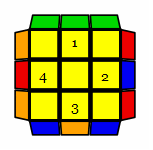
\includegraphics[scale=2]{numbered.png}
\begin{enumerate}
    \item The U perm (specifically Ub) can be executed using the algorithm R2 U R U R' U' R3 U' R' U R' and permutes the edges as shown in the image below. Write the operation of the U perm in cycle notation, in the form 
    $\begin{pmatrix}
    1 & 2 & 3 & 4\\
    a & b & c & d
    \end{pmatrix}$, where a through d are numbers from 1 through 4.\\
    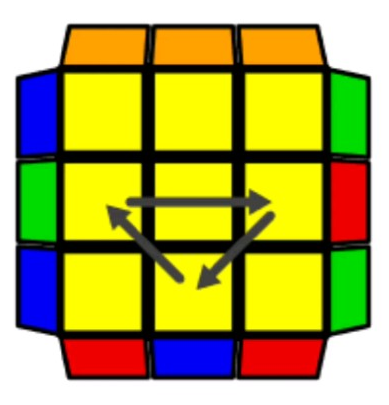
\includegraphics[scale=0.5]{uperm.png}\\
    We can model this as the permutation 
    $\begin{pmatrix}
    1 & 2 & 3 & 4\\
    1 & 3 & 4 & 2
    \end{pmatrix}$, since the piece labelled "1" stays in the same spot, and the pieces 2, 3, and 4 cycle.
    
    \item The H perm can be executed using the algorithm M2 U M2 U2 M2 U M2 and permutes the edges as shown in the image below. Write the operation of the H perm in the same format as the previous question. \\
    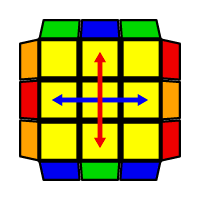
\includegraphics[scale=0.3]{hperm.png}\\
    $\begin{pmatrix}
    1 & 2 & 3 & 4\\
    3 & 4 & 1 & 2
    \end{pmatrix}$
    
    \item Consider the composition of the H perm and the U perm, given by $H\circ U$ (first you do U perm, then you do H perm). Write the operation of this function in cycle notation as before. \\
    $\begin{pmatrix}
    1 & 2 & 3 & 4\\
    3 & 1 & 2 & 4
    \end{pmatrix}$\\
    An easiest way to see this is to track each piece individually through both permutations. We have 1 staying the same during U perm, then going to 3 in H perm. So the composition gives 1 goes to 3. We can continue the same process for the other pieces. Alternatively, we could just execute the algorithms on our cube to see the same thing.
\end{enumerate}

\newpage
\section{Homework 5}
\begin{enumerate}
    \item Write the following permutation (given in two-line notation) in one-line notation: $\begin{pmatrix}
    1 & 2 & 3 & 4 & 5 & 6\\
    1 & 3 & 2 & 5 & 6 & 4
    \end{pmatrix}$\\
    (2 3)(4 5 6). We can interchange the two cycles and the permutation is the same.
    \item Consider the J-perm given as R U R' F' R U R' U' R' F R2 U' R' U'. You can see how the cube looks after the algorithm here (Links to an external site.). Identify the parity of the corners and the parity of the edges, separately.\\
    Both the corners and edges have odd parity. The edges can be solved with a single transposition (swap), making the parity odd. The same can be said for the edges.
    
    \item Give the inverse of the following permutation (written in one-line cycle notation): (3 2 1)(4 5)(7 9 8 10). \\
    (1 2 3)(5 4)(10 8 9 7). We can invert by simply reversing each sequence. The order of the cycles does not matter.
\end{enumerate}


\end{document}